\documentclass[aspectratio=169]{beamer}
%la opcion hangout es para complilar en modo imprimible
%\documentclass[hangout]{beamer}

\mode<presentation>
{
  \usetheme{Berkeley}
  \setbeamercovered{transparent}
  \setbeamertemplate{navigation symbols}{}
}

\usepackage[spanish]{babel}
\usepackage[utf8]{inputenc}
\usepackage{tikz}
\usepackage{textpos}
\usepackage{hyperref}

%\usetikzlibrary{shapes,arrows}
\setbeamerfont{author}{size=\large}
\setbeamerfont{institute}{size=\normalsize\bfseries}
\setbeamerfont{title}{size=\Large\bfseries}
\setbeamerfont{subtitle}{size=\huge}

\definecolor{darkblue}{RGB}{51,51,179}

\title[802.15.4 LR-WPAN]{Protocolos de Comunicación en Sistemas Embebidos}
\subtitle{802.15.4 LR-WPAN}
\author[]{Ing. Patricio Bos, Esp. Ing. Juan Montilla}
\institute[CESE-FIUBA]{Carrera de Especialización en Sistemas Embebidos - FIUBA}
\date{}

%\subtitle{Framework para aplicaciones de control de ambientes}
\titlegraphic{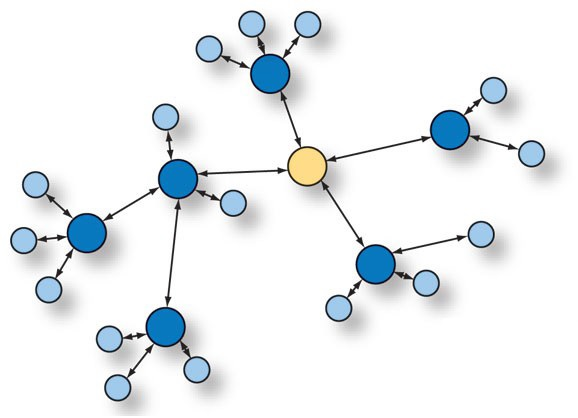
\includegraphics[width=5cm]{./imagenes/red.jpg}}


\subject{Protocolos y Comunicaciones: 802.15.4 LR-WPAN. Carrera de Especialización en Sistemas Embebidos}
% This is only inserted into the PDF information catalog. Can be left
% out. 

\pgfdeclareimage[height=1.5cm]{university-logo}{./imagenes/logo-facu-inverso.png}
\logo{\pgfuseimage{university-logo}}


% If you wish to uncover everything in a step-wise fashion, uncomment
% the following command: 

\beamerdefaultoverlayspecification{<+->}
  
\begin{document}

%la magia del begingroup es para que titlepage quede centrada, sin eso queda
%corrida en el ancho del sidebar
\begingroup
\makeatletter
\setlength{\hoffset}{-.5\beamer@sidebarwidth}
\makeatother
\begin{frame}[plain,noframenumbering]
  \titlepage
\end{frame}

\endgroup

\setbeamertemplate{caption}{\raggedright\insertcaption\par}


\begin{frame}{\textbf{Organización de la presentación}}
  \tableofcontents
  % You might wish to add the option [pausesections]
\end{frame}
%
%

%-------------------------------------------------%
%-------------------------------------------------%
\section{Introducción}
%-------------------------------------------------%
%-------------------------------------------------%

%-------------------------------------------------%
\subsection[IEEE 802]{Grupo de trabajo IEEE 802}
%-------------------------------------------------%


\begin{frame}{Grupos de trabajo IEEE} 

\begin{minipage}[c]{1.0\linewidth}
	\begin{minipage}[c]{0.6\linewidth}
		\begin{itemize}
			\item IEEE 802: Desarrollar estándares para redes de área local y metropolitana (LAN y MAN)
			\begin{itemize}
				\item IEEE 802.3: Ethernet
				\item IEEE 802.11: Wi-fi
				\item ...
			\end{itemize}
			\vspace{10px}
			\item IEEE 802.15: Redes inalámbricas de área personal (WPAN)
			\vspace{5px}
			\begin{itemize}
				\item IEEE 802.15.1: Bluetooth
				\item IEEE 802.15.4: WPANs de baja tasa de transferencia de datos (LR-WPAN)
			\end{itemize}
		\end{itemize}
	\end{minipage}
	\begin{minipage}[c]{0.35\linewidth}
		\begin{figure}[H]
			\uncover<2>{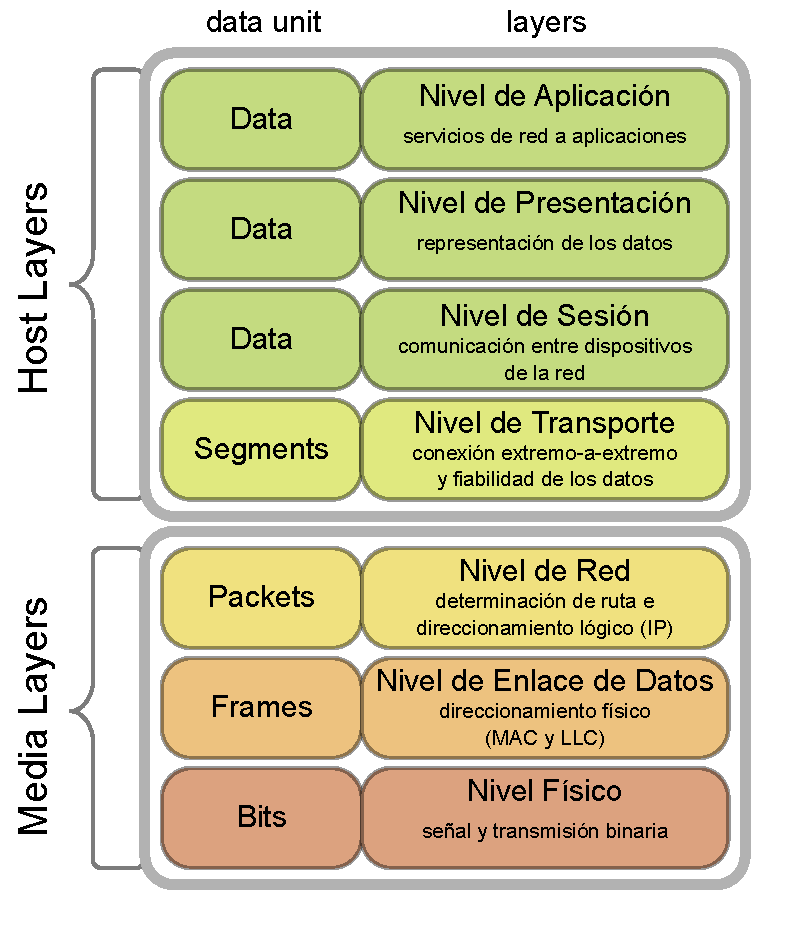
\includegraphics[width=1\textwidth]{./imagenes/OSI_Model_v1.pdf}}
			\label{OSI_model}
			%\caption{Modelo de capas OSI}
		\end{figure}	  	  	
	\end{minipage}
\end{minipage}
	
\end{frame}

%-------------------------------------------------%
\subsection[IEEE 802.15.4]{IEEE 802.15.4 LR-WPAN}
%-------------------------------------------------%

\begin{frame}{IEEE 802.15.4}{LR-WPAN}
	\begin{itemize}
		\item Versiones: 802.15.4:2003, 802.15.4:2006 y \textbf{802.15.4:2011}
		\vspace{5px}
		\item Define:
		\begin{itemize}
			\item Nivel físico (PHY)
			\item Control de acceso al medio (MAC)
		\end{itemize}
		\vspace{5px}
		\item Características:
		\begin{itemize}
			\item Comunicaciones simples de bajo costo. 
			\item Bajas tasas de transferencia (throughput).
			\item Para aplicaciones con limitaciones de potencia.
			\item Confiabilidad en la transferencia de datos.
			\item Opera en una banda de frecuencia sin licencia.
		\end{itemize}
	\end{itemize}
	
\end{frame}

\begin{frame}{IEEE 802.15.4}{Características Generales}
	
	\begin{itemize}
		\item Área de operación: 10m
		\vspace{5px}
		\item Tasa de transferencia: 250kbs
		\vspace{5px}
		\item Adecuación a aplicaciones de tiempo real: \textit{Guaranteed Time Slots} (GTSs)
		\vspace{5px}
		\item Mecanismo para evitar colisiones:\\ \textit{Carrier Sense Multiple-Access / Collision Avoidance} (CSMA/CA)
		\vspace{5px}
		\item Control de consumo de energía: 
		\begin{itemize}
			\item \textit{Link Quality Indicator} (LQI)
			\item \textit{Energy Detection} (ED)
		\end{itemize}
	\end{itemize}
	
\end{frame}


%-------------------------------------------------%
%-------------------------------------------------%
\section{LR-WPAN}
%-------------------------------------------------%
%-------------------------------------------------%

%-------------------------------------------------%
\subsection[Dispositivos]{Tipos de Dispositivos}
%-------------------------------------------------%

\begin{frame}{Componentes}{Tipos de dispositivos}
% El primer minipage es un marco para las otras dos, que parten la pantalla en dos horizontalmente.
% Con 0.6\linewidth le indicás que porcentaje del ancho de la página debe tener la minipage
\begin{minipage}[c]{1.0\linewidth}
	\begin{minipage}[c]{0.5\linewidth}
		\begin{itemize}
			\item Full-function device (FFD):\\ Capaz de ser PAN coordinator o coordinator. 
			\vspace{10px}
			\item Reduced-function device (RFD):\\ Sólo puede comunicarse con un FFD. Requerimientos mínimos de recursos.
			%\vspace{10px}
	  	\end{itemize}	
	\end{minipage}	
	\begin{minipage}[c]{0.5\linewidth}
		\begin{figure}
			\begin{align*} 
				{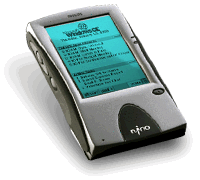
\includegraphics[width=.3\textwidth]{./imagenes/FFD}}
				\hspace{15px} 
				{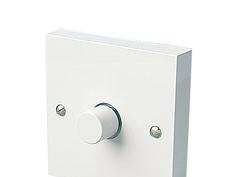
\includegraphics[width=.35\textwidth]{./imagenes/RFD}}
				\end{align*}\\
				\vspace{15px}
				{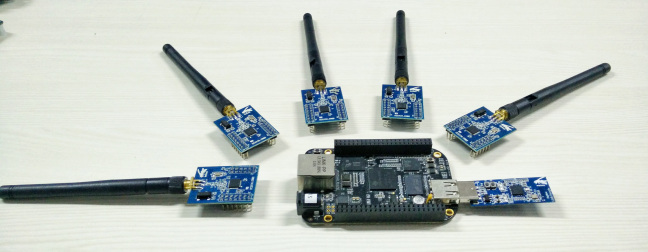
\includegraphics[width=.6\textwidth]{./imagenes/FFDvsRFD}}
			
		\end{figure}	  	  	  	
	\end{minipage}	
\end{minipage}
\end{frame}

%-------------------------------------------------%
\subsection[Topología]{Topología de la red}
%-------------------------------------------------%

\begin{frame}{Topología de la Red}{Estrella o punto a punto}

\begin{minipage}[c]{1.0\linewidth}
	\begin{minipage}[c]{0.45\linewidth}
		\begin{itemize}
			\item Estrella (Star)
			\begin{itemize}
				\item PAN coordinator.
				\item Comunicaciones centralizadas.
				\item Ej: Automatización del hogar, Periféricos de PC, Juegos,...
					\end{itemize}
			\vspace{10px}
			\item Punto a punto (Peer-to-Peer)
			\begin{itemize}
				\item PAN coorditator.
				\item Permite redes más complejas.
				\item Multi-Hop routing.
				\item Ej: Control industrial,  WSNs, Tracking de inventario,...
			\end{itemize}
	  	\end{itemize}	
	\end{minipage}
	\hspace{-20px}
	\begin{minipage}[c]{0.7\linewidth}
		\begin{figure}[H]
			{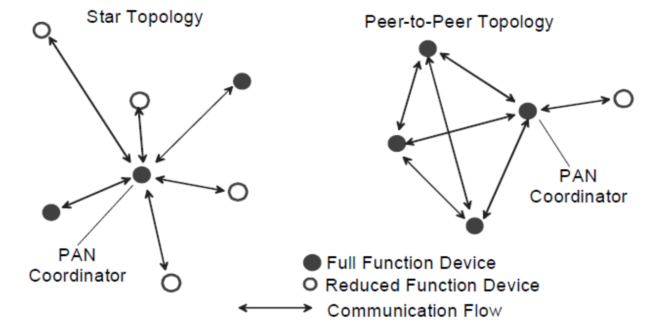
\includegraphics[width=.7\textwidth]{./imagenes/Topology}}
		\end{figure}	  	  	
	\end{minipage}
\end{minipage}
\end{frame}

\begin{frame}{Topología Punto a punto}{Árbol de Cluster}
\begin{minipage}[c]{1.0\linewidth}
\begin{minipage}[c]{0.45\linewidth}
		\begin{itemize}
			\item Mayoría de FFDs.
			\vspace{10px}
			\item 1 \textit{overall PAN coordinator}.
			\vspace{10px}
			\item RFDs al final de una rama.
			\vspace{10px}
			\item Aumenta el área de covertura.
			\vspace{10px}
			\item Aumenta la latencia de la red.
		\end{itemize}	
	\end{minipage}
	\hspace{-15px}
	\begin{minipage}[c]{0.65\linewidth}
		\begin{figure}[H]
			{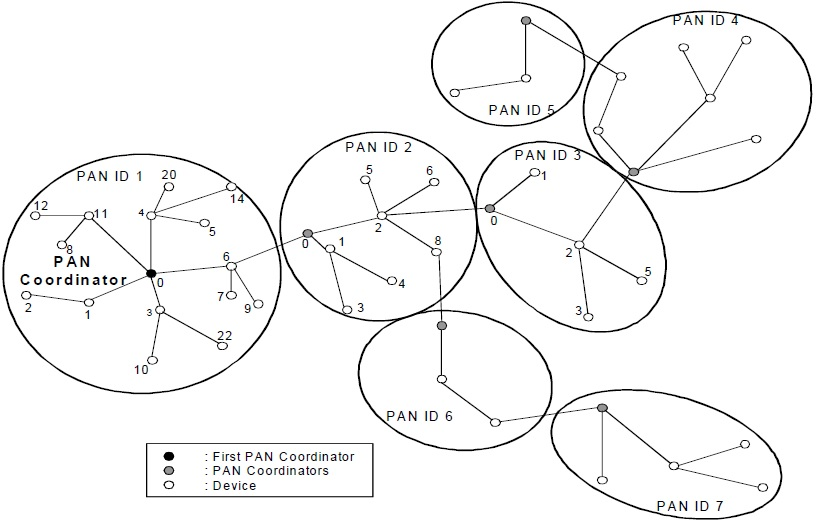
\includegraphics[width=.8\textwidth]{./imagenes/cluster}}
		\end{figure}	  	  	
	\end{minipage}
\end{minipage}
\end{frame}

%-------------------------------------------------%
\subsection[Arquitectura]{Arquitectura del estándar}
%-------------------------------------------------%

\begin{frame}{Arquitectura del estándar}

\begin{minipage}[c]{1.0\linewidth}
	\begin{minipage}[c]{0.6\linewidth}
		\begin{itemize}
			\item MAC Sublayer
			\begin{itemize}
				\item Beacon management
				\item Channel access
				\item GTSs management
				\item Frame validation, ACKs
				\item Asociación y desasociación de dispositivos
			\end{itemize}
			\vspace{10px}
			\item Physical Layer (PHY):
			\begin{itemize}
				\item Activación/Desactivación de RF
				\item ED, LQI, Clear Channel Assessment (CCA)
				\item Channel selection
				\item Tx y Rx de paquetes a través del medio físico
			\end{itemize}
			\vspace{10px}
		\end{itemize}	
	  \end{minipage}
	  \begin{minipage}[c]{0.35\linewidth}
		\begin{figure}[H]
			{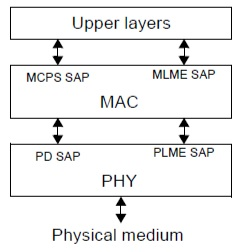
\includegraphics[width=.6\textwidth]{./imagenes/arquitectura}}
		\end{figure}	  	  	
	  \end{minipage}
\end{minipage}

\end{frame}


\begin{frame}[t]{MAC: Beacons, Supertramas y GTSs}
\begin{minipage}[c]{1.0\linewidth}
\begin{minipage}[c]{0.35\linewidth}
		\begin{itemize}
			\item 16 time slots.
			\vspace{5px}
			\item Contention Access Period (CAP)\\ \textbf{con CSMA/CA}.
			\vspace{5px}
			\item Contention Free Period (CFP) para los GTSs, \textbf{sin CSMA/CA}.
			\vspace{5px}
			\item Los GTSs son opcionales y reducen el CAP.
			\vspace{5px}
			\item Tiempo inactivo $\rightarrow$ modo bajo consumo.
		\end{itemize}	
	\end{minipage}
%	\hspace{-5px}
	\begin{minipage}[c]{0.65\linewidth}
		\begin{figure}[H]
			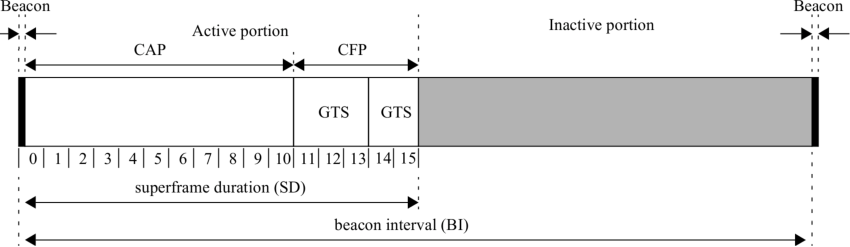
\includegraphics[width=1\linewidth]{./imagenes/superFrame}\\
		\end{figure}	  	  	
	\end{minipage}
\end{minipage}
%\vspace{10px}
%	\begin{figure}[H]
%		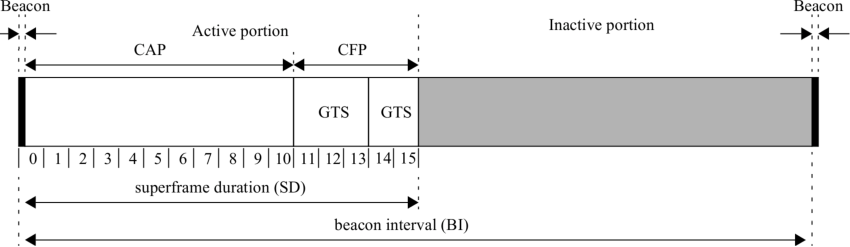
\includegraphics[height=.35\textheight]{./imagenes/superFrame}\\
%	\end{figure}

\end{frame}

%--------------------------------------------------------------------%
\subsection[Transferencia de datos]{Modelo de Transferencia de datos}
%--------------------------------------------------------------------%


\begin{frame}[t]{Transferencia de Datos}
\textbf{Con beacon}
%\vspace{10px}
\begin{columns}[t]
	\begin{column}{.5\textwidth}
		\begin{minipage}[t][0.7\textheight][s]{\columnwidth}
			\begin{figure}[H]
				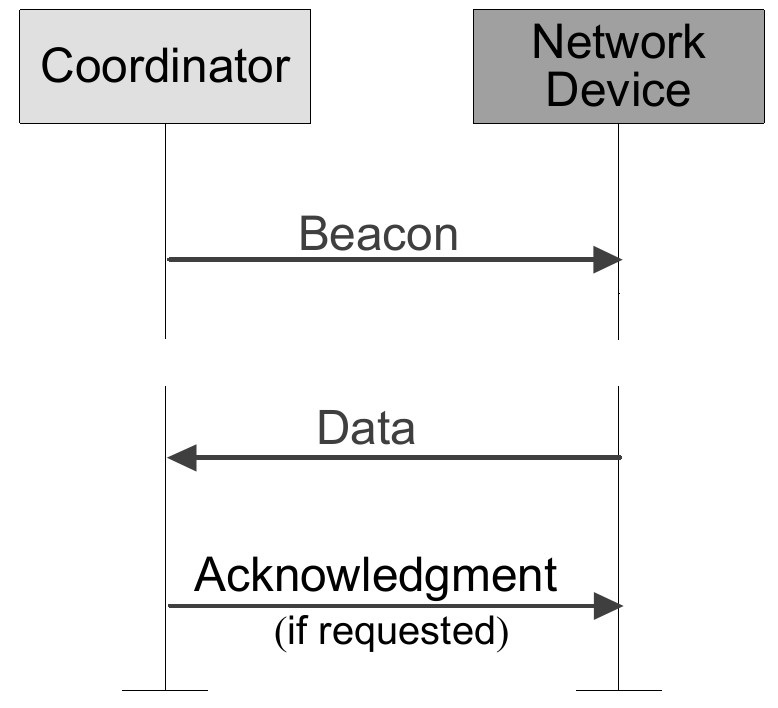
\includegraphics[height=.65\textheight]{./imagenes/dev-coord-beacon.jpg}
				\vfill
				\vspace{10px}
				\caption{Device $\rightarrow$ Coordinator}
			\end{figure}
		\end{minipage}
	\end{column}
	\begin{column}{.5\textwidth}
		\begin{minipage}[t][0.7\textheight][s]{\columnwidth}
			\begin{figure}[H]
				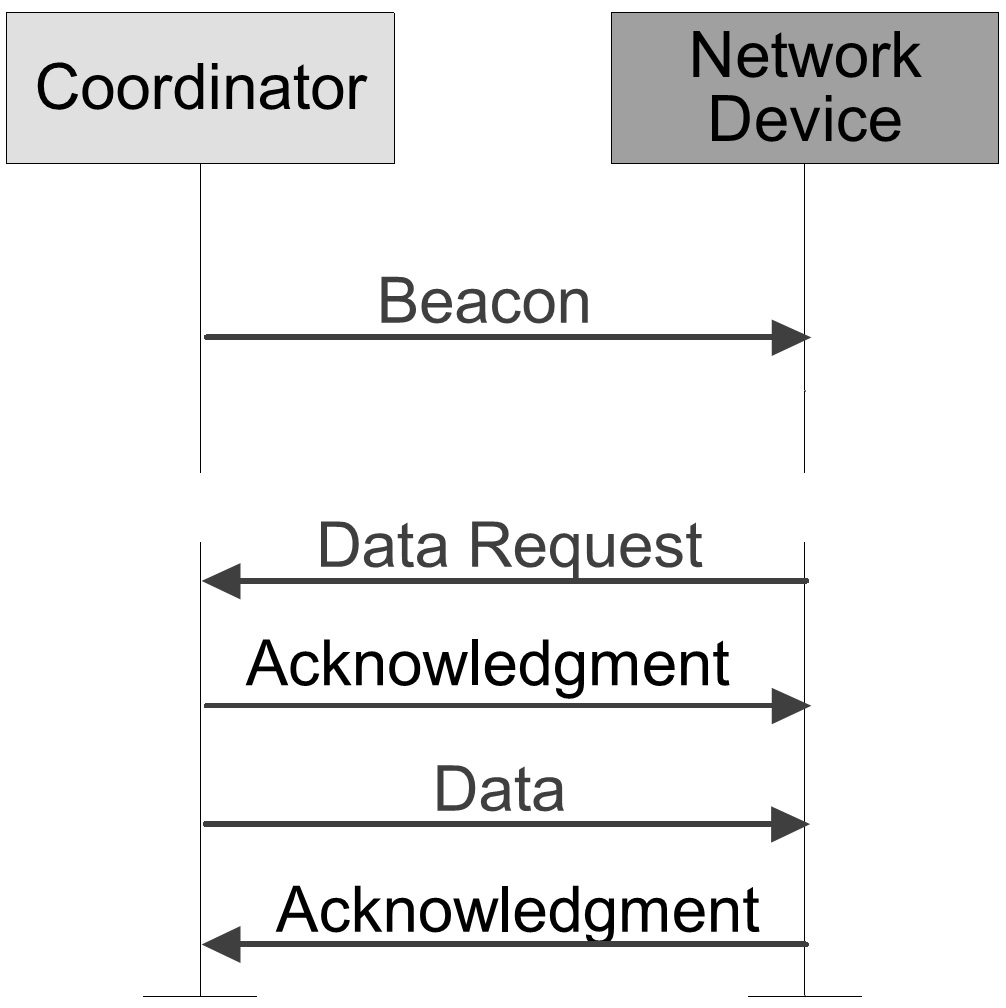
\includegraphics[height=.7\textheight]{./imagenes/coord-dev-beacon.jpg}
				\vfill
				\caption{Coordinator $\rightarrow$ Device}
			\end{figure}	 		
		\end{minipage}
	\end{column}
\end{columns}
\end{frame}

\begin{frame}[t]{Transferencia de Datos}
\textbf{Sin beacon}
%\vspace{10px}
\begin{columns}[t]
	\begin{column}{.5\textwidth}
		\begin{minipage}[t][0.7\textheight][s]{\columnwidth}
			\begin{figure}[H]
				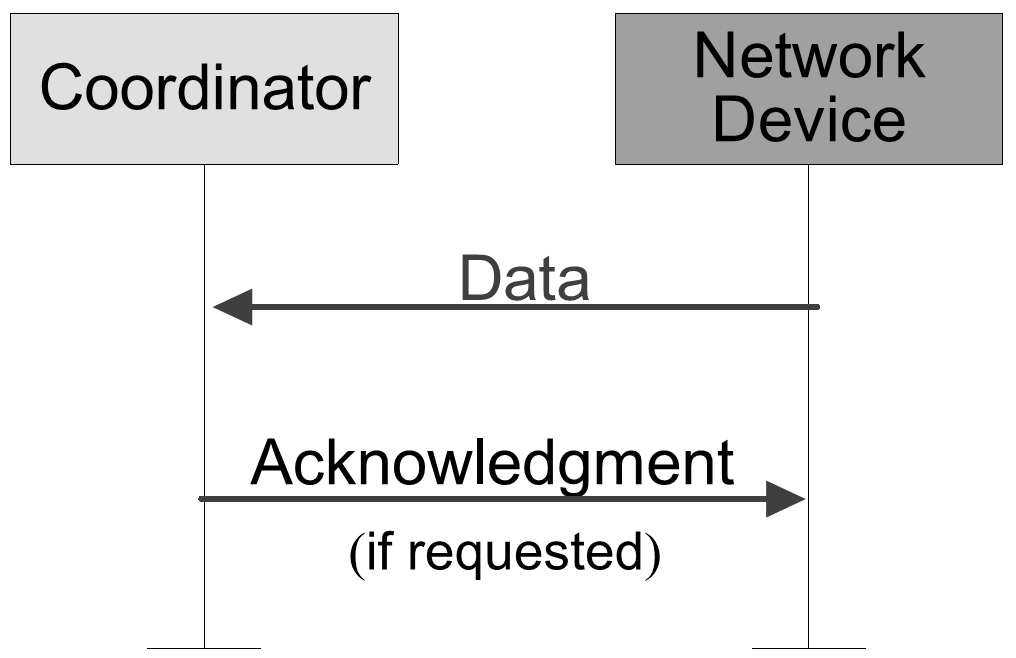
\includegraphics[height=.45\textheight]{./imagenes/dev-coord-sinbeacon.jpg}
				\vfill
				\vspace{10px}
				\caption{Device $\rightarrow$ Coordinator}
			\end{figure}
		\end{minipage}
	\end{column}
	\begin{column}{.5\textwidth}
		\begin{minipage}[t][0.7\textheight][s]{\columnwidth}
			\begin{figure}[H]
				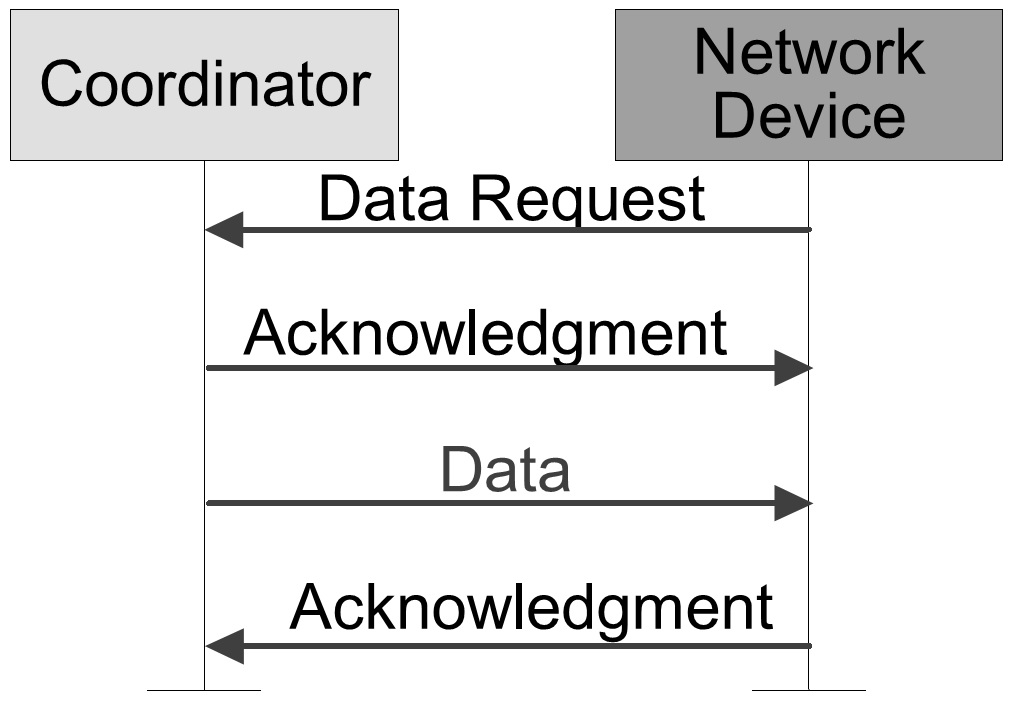
\includegraphics[height=.5\textheight]{./imagenes/coord-dev-sinbeacon.jpg}
				\vfill
				\caption{Coordinator $\rightarrow$ Device}
			\end{figure}	 		
		\end{minipage}
	\end{column}
\end{columns} 	  	
\end{frame}


%--------------------------------------------------------------------%
\subsection[Tramas]{Estructura de las Tramas}
%--------------------------------------------------------------------%

\begin{frame}{Estructura de las Tramas}
Se definen 4 tipos de trama MAC:
\vspace{5px}
	\begin{itemize}
		\item Beacon
		\vspace{5px}
		\item Data
		\vspace{5px}
		\item Acknowledge
		\vspace{5px}
		\item MAC Command
		\vspace{5px}
	\end{itemize}
	\begin{figure}[H]
		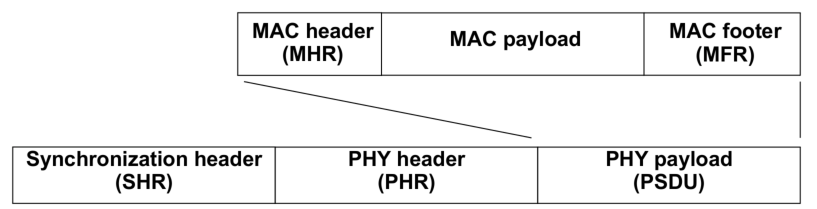
\includegraphics[width=1\textwidth]{./imagenes/frameStructure}
	\end{figure}	 	
\end{frame}

\begin{frame}[t]{Tramas}
Tipo de Frame: \textbf{Beacon}
\vspace{10px}
	\begin{figure}[H]
		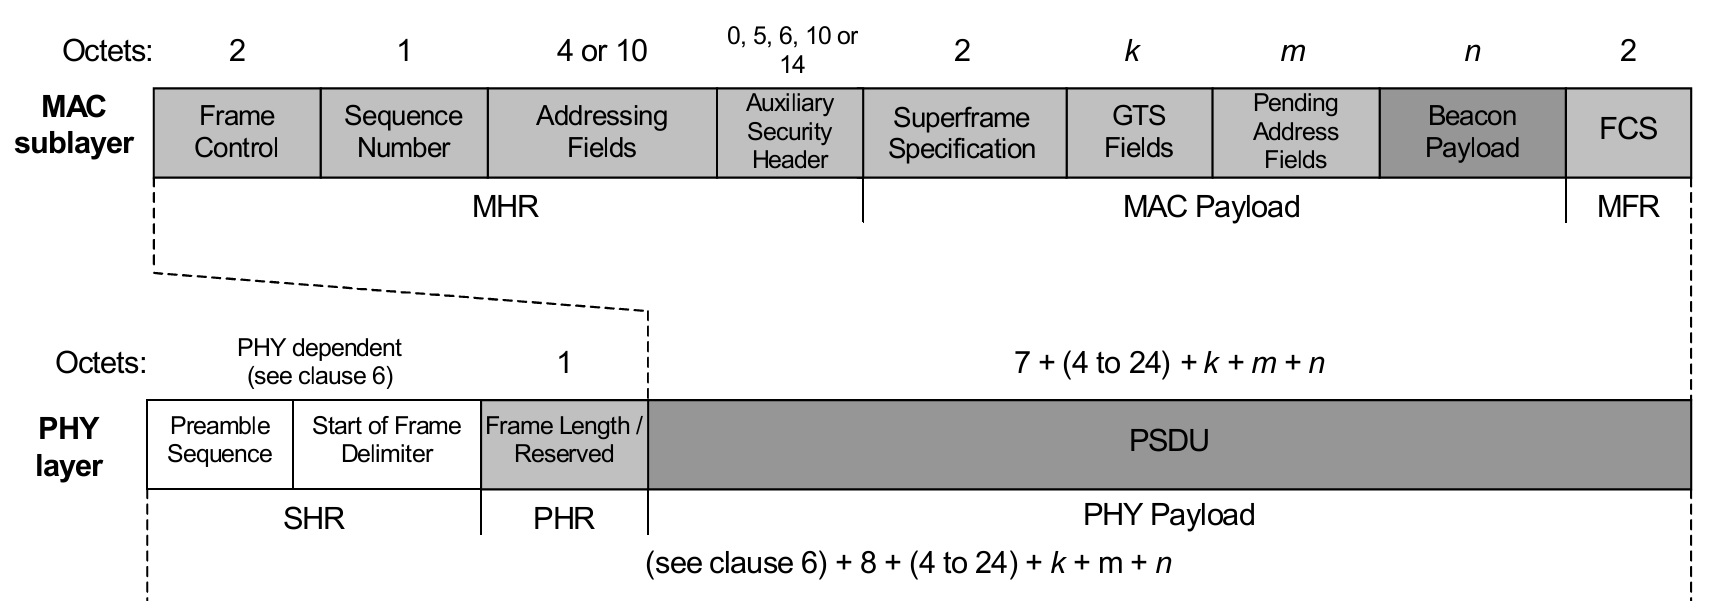
\includegraphics[width=1\textwidth]{./imagenes/beacon.jpg}
	\end{figure}	  	  	
\end{frame}

\begin{frame}[t]{Tramas}
Tipo de Frame: \textbf{Data}
\vspace{10px}
	\begin{figure}[H]
		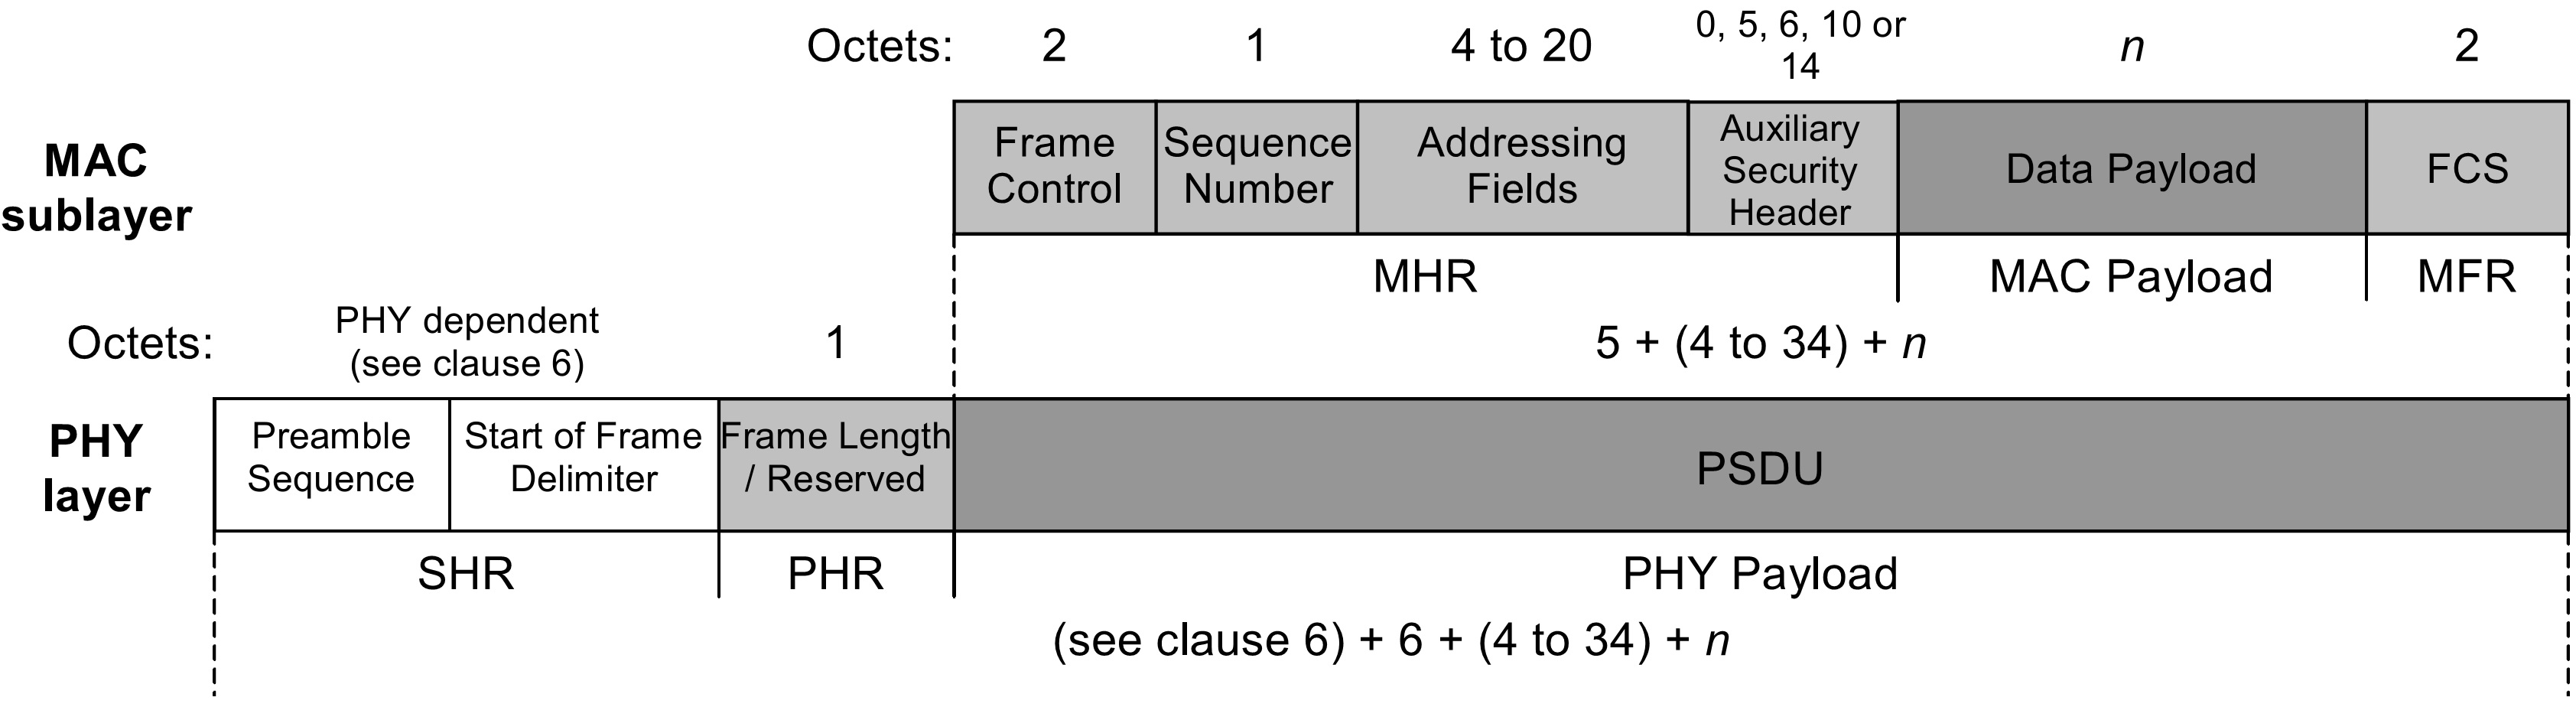
\includegraphics[width=1\textwidth]{./imagenes/data.jpg}
	\end{figure}	  	  	
\end{frame}


\begin{frame}[t]{Tramas}
Tipo de Frame: \textbf{Acknowledgement} (Ack)
\vspace{10px}
	\begin{figure}[H]
	\centering
		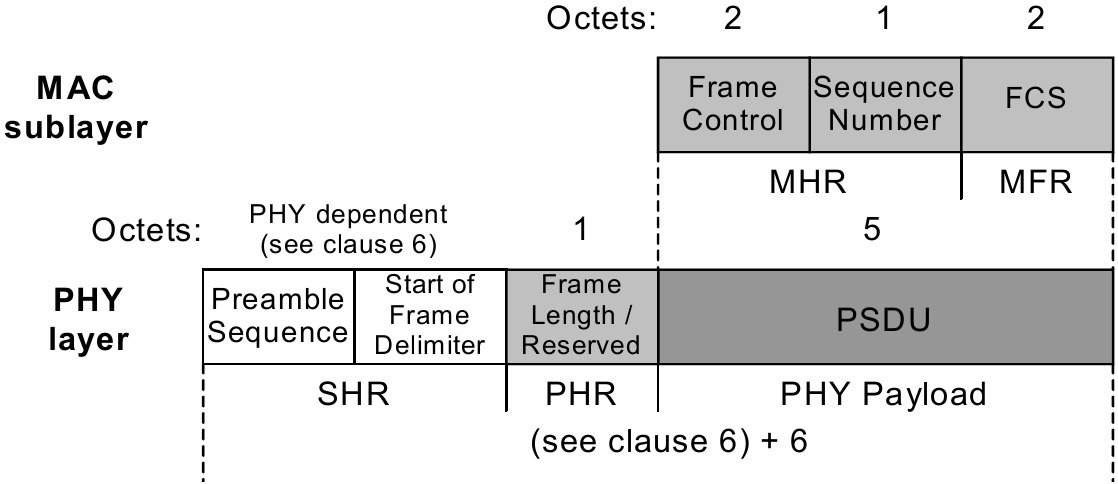
\includegraphics[width=.8\textwidth]{./imagenes/ack.jpg}
	\end{figure}	  	  	
\end{frame}

\begin{frame}[t]{Tramas}
Tipo de Frame: \textbf{MAC Command}
\vspace{10px}
	\begin{figure}[H]
		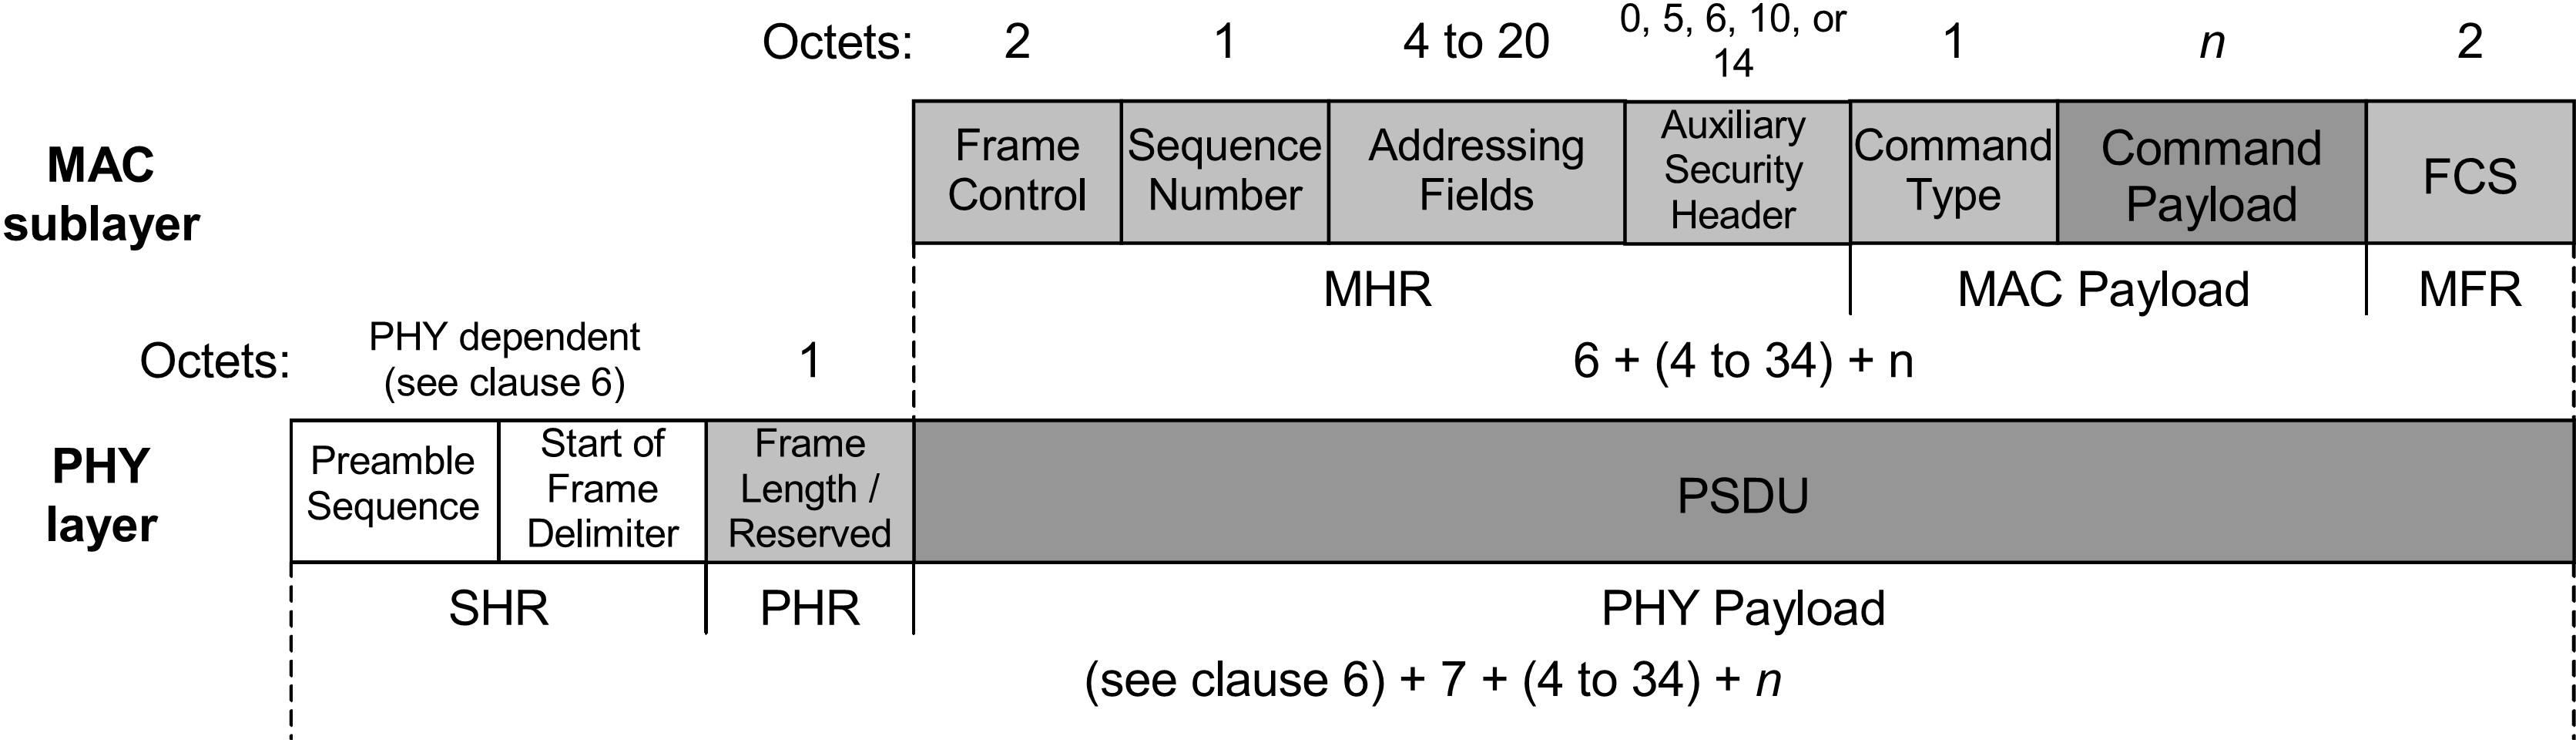
\includegraphics[width=1\textwidth]{./imagenes/maccommand.jpg}
	\end{figure}	  	  	
\end{frame}


\begin{frame}[t]{Tramas}
Frame Control Field
	\begin{figure}[H]
	\centering
		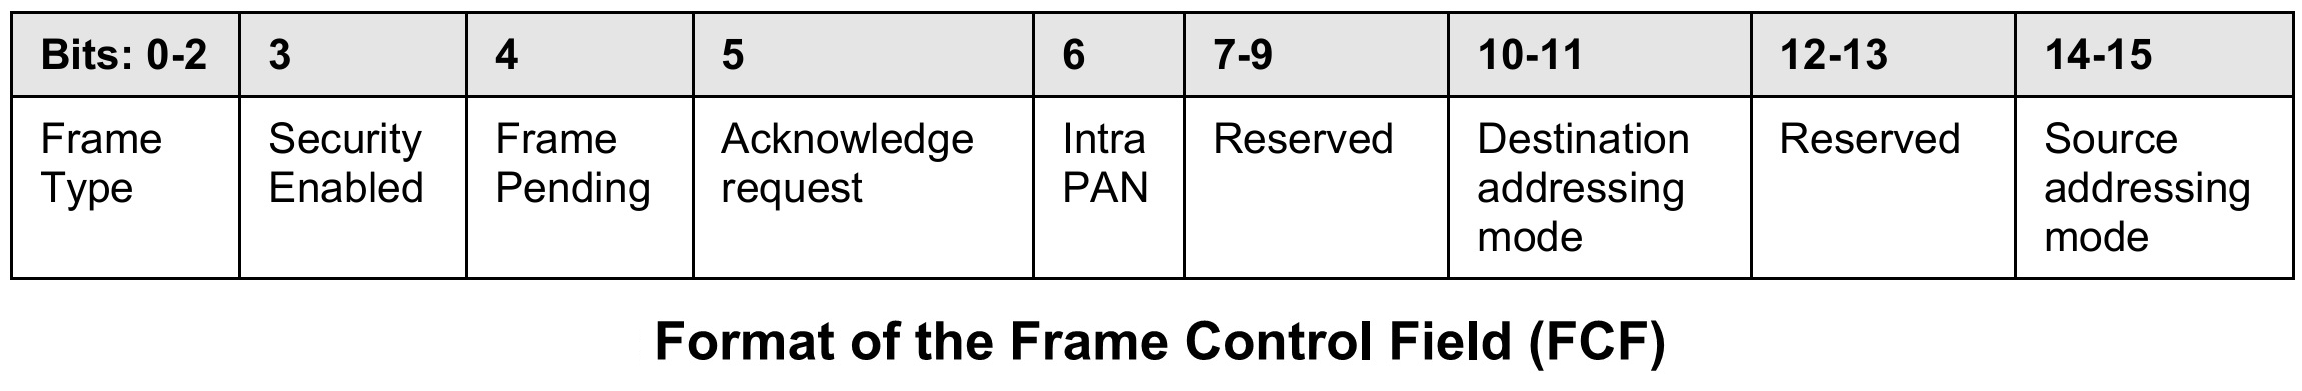
\includegraphics[height=.3\textheight]{./imagenes/FCF.jpg}\\
		\vspace{20px}
		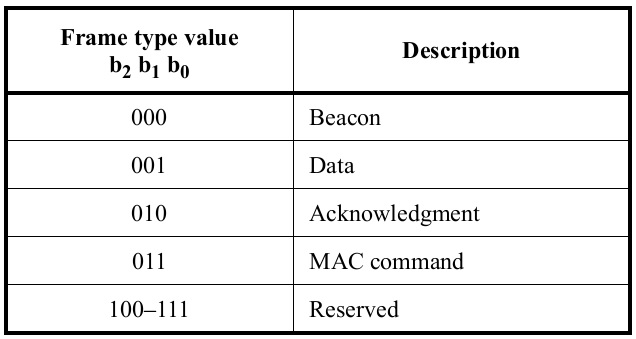
\includegraphics[height=.3\textheight]{./imagenes/frametype.jpg}
		\hspace{20px} 
		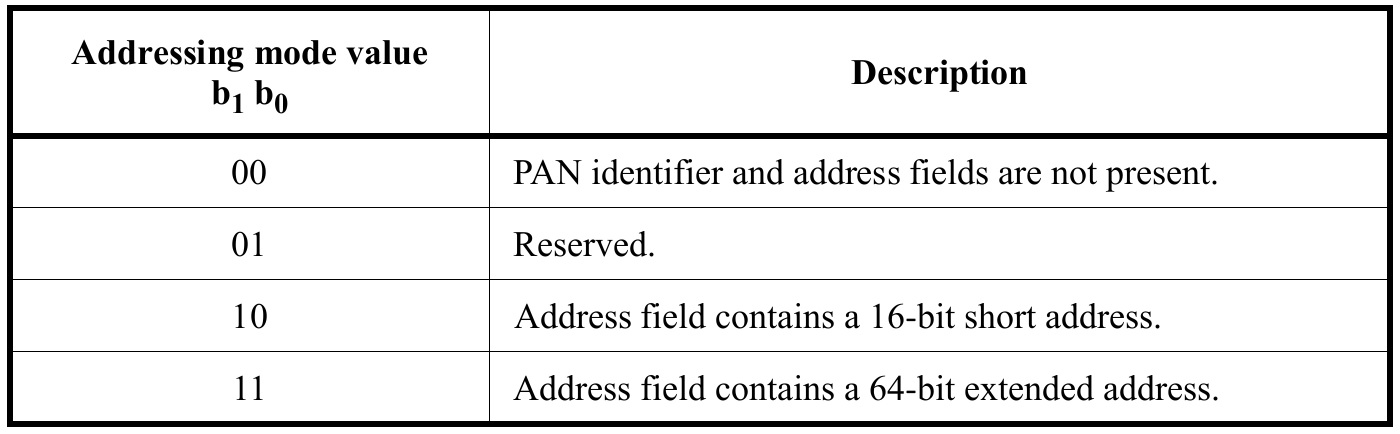
\includegraphics[height=.3\textheight]{./imagenes/addressingmode.jpg}
	\end{figure} 	
\end{frame}

%%%%%%%%%%%%%%%%%%%%%%%%%%%%%%%%%%%%%%%%%%%%%%
%@JUAN: ESTO NO SE CÓMO LO VAMOS A EXPLICAR!!!
%%%%%%%%%%%%%%%%%%%%%%%%%%%%%%%%%%%%%%%%%%%%%%
%--------------------------------------------------------------------%
\subsection[CSMA]{CSMA}
%--------------------------------------------------------------------%

\begin{frame}[T]{Control de Acceso al Medio}

Slotted CSMA/CA vs Unslotted CSMA/CA
\vspace{10px}
		\begin{figure}[H]
			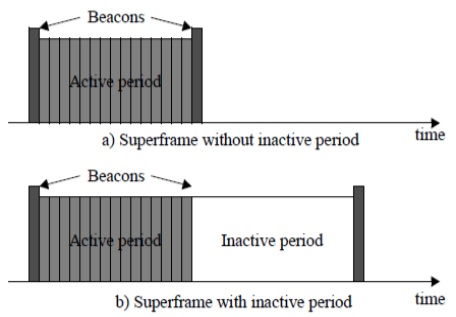
\includegraphics[height=.4\textheight]{./imagenes/superframe.jpg}\\
			\vspace{15px}
			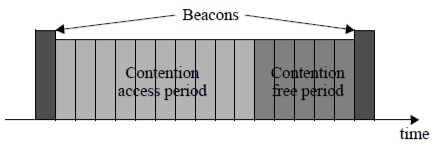
\includegraphics[height=.3\textheight]{./imagenes/unsolotted.jpg}
		\end{figure}
\end{frame}

%--------------------------------------------------------------------%
\subsection[Modulación]{Modulación}
%--------------------------------------------------------------------%

\begin{frame}{\textbf{Modulación}}
%\fontsize{14pt}{15}\selectfont
\begin{minipage}[c]{1.0\linewidth}
\begin{figure}[H]
	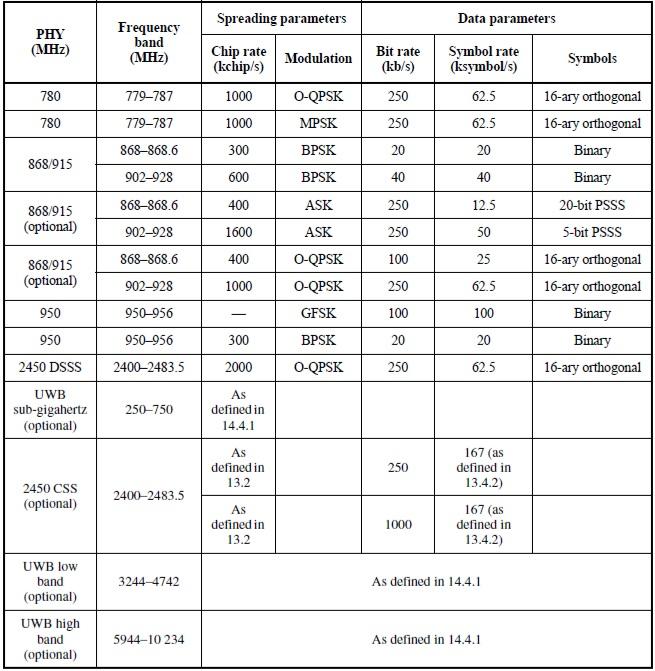
\includegraphics[height=1\textheight]{./imagenes/modulaciones.jpg}
		\end{figure}	
\end{minipage}
\end{frame}

%-------------------------------------------------%
%-------------------------------------------------%
\section{Mote LSE}
%-------------------------------------------------%
%-------------------------------------------------%

%-------------------------------------------------%
\subsection[Mote]{Mote}
%-------------------------------------------------%
\begin{frame}{Nodo Mote LSE-FIUBA} 

\begin{minipage}[c]{1.0\linewidth}
	\begin{minipage}[c]{0.6\linewidth}
		\begin{itemize}
			\item Nodo Mote desarrollado en el LSE-FIUBA
			\vspace{15px}
			\begin{itemize}
				\item Placa LPC1343 con procesador ARM Cortex-M3 de 32 bits
				\vspace{5px}
				\item 32 KB de flash
				\vspace{5px}
				\item 8 KB de SRAM
				\vspace{5px}
				\item Frecuencia de reloj de 72 MHz
			\end{itemize}
			\vspace{10px}
		\end{itemize}
	\end{minipage}
	\begin{minipage}[c]{0.35\linewidth}
		\begin{figure}[H]
			\uncover<2>{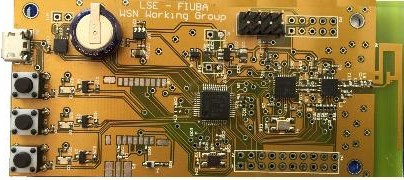
\includegraphics[width=1\textwidth]{./imagenes/mote.jpg}}
			\label{Mote LSE}
			%\caption{Mote LSE}
		\end{figure}	  	  	
	\end{minipage}
\end{minipage}
\end{frame}

%-------------------------------------------------%
\subsection[TI CC2520]{TI CC2520}
%-------------------------------------------------%
\begin{frame}{Transceptor DSSS TI CC2520} 
\begin{minipage}[c]{1.0\linewidth}
	\begin{minipage}[c]{0.6\linewidth}
		\begin{itemize}
			\item 2394-2507 MHz	
			\item VCO, LNA, PA y filtros On-chip	
			\item 3 modos de potencia flexibles para consumo reducido
			\item Muy bajo consumo de corriente
			\begin{itemize}
				\item RX: 18.5 - 22.3 mA.
				\item TX: 25.8 - 33.6 mA.
			\end{itemize}
			\item Interfaz de usuario
			\begin{itemize}
				\item 4 SPI
				\item 6 GPIO
				\item Generador de interupciones
				\item Control de respuestas automáticas a diferentes eventos
				\item Modo de Packet Sniffer embebido
			\end{itemize}
			\vspace{10px}
		\end{itemize}
	\end{minipage}
	\begin{minipage}[c]{0.35\linewidth}
		\begin{figure}[H]
			\uncover<2>{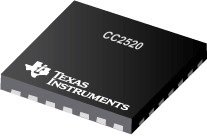
\includegraphics[width=1\textwidth]{./imagenes/cc2520.jpg}}
			\label{cc2520}
			%\caption{cc2520}
		\end{figure}	  	  	
	\end{minipage}
\end{minipage}
\end{frame}

\begin{frame}{\textbf{Circuito de Aplicación Típico}}	
	\begin{figure}[H]
		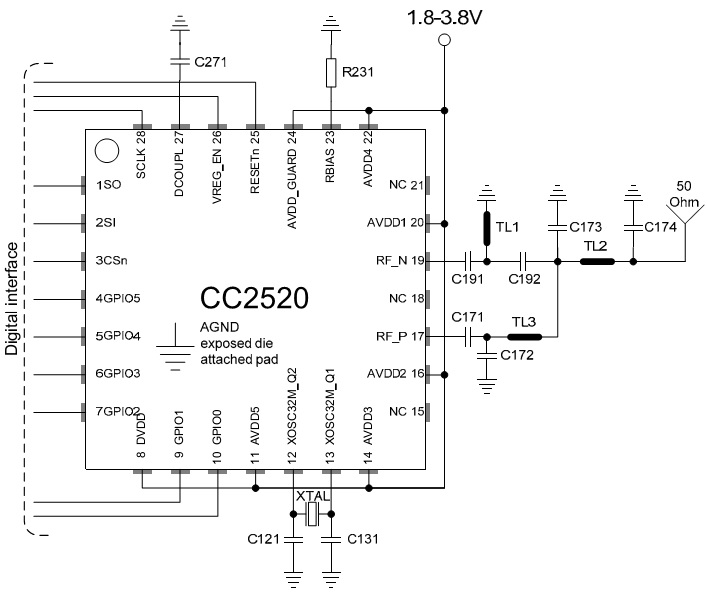
\includegraphics[height=1\textheight]{./imagenes/applicationcircuit.jpg}
	\end{figure}	
\end{frame}

\begin{frame}{Soporte por Hardware a 802.15.4 MAC} 
\begin{minipage}[c]{1.0\linewidth}
	\begin{minipage}[c]{0.6\linewidth}
		\begin{itemize}
			\item Generador automático de preámbulo	
			\item Inserción y detección de palabra de sincronización	
			\item CRC-16 en el MAC payload
			\item Frame Filtering
			\item Ack automático
			\item Clear Channle Assessment (CCA)
			\item Energy detection / RSSI
			\item Link Quality Indication (LQI)
			\item Seguridad MAC automática (CTR, CBC-MAC,CCM)
			\vspace{10px}
		\end{itemize}
	\end{minipage}
	\begin{minipage}[c]{0.35\linewidth}
		\begin{figure}[H]
			\uncover<2>{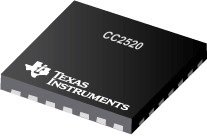
\includegraphics[width=1\textwidth]{./imagenes/cc2520.jpg}}
			\label{cc2520}
			%\caption{cc2520}
		\end{figure}	  	  	
	\end{minipage}
\end{minipage}
\end{frame}

\begin{frame}{\textbf{Diagrama Funcional}}

	\begin{figure}[H]
		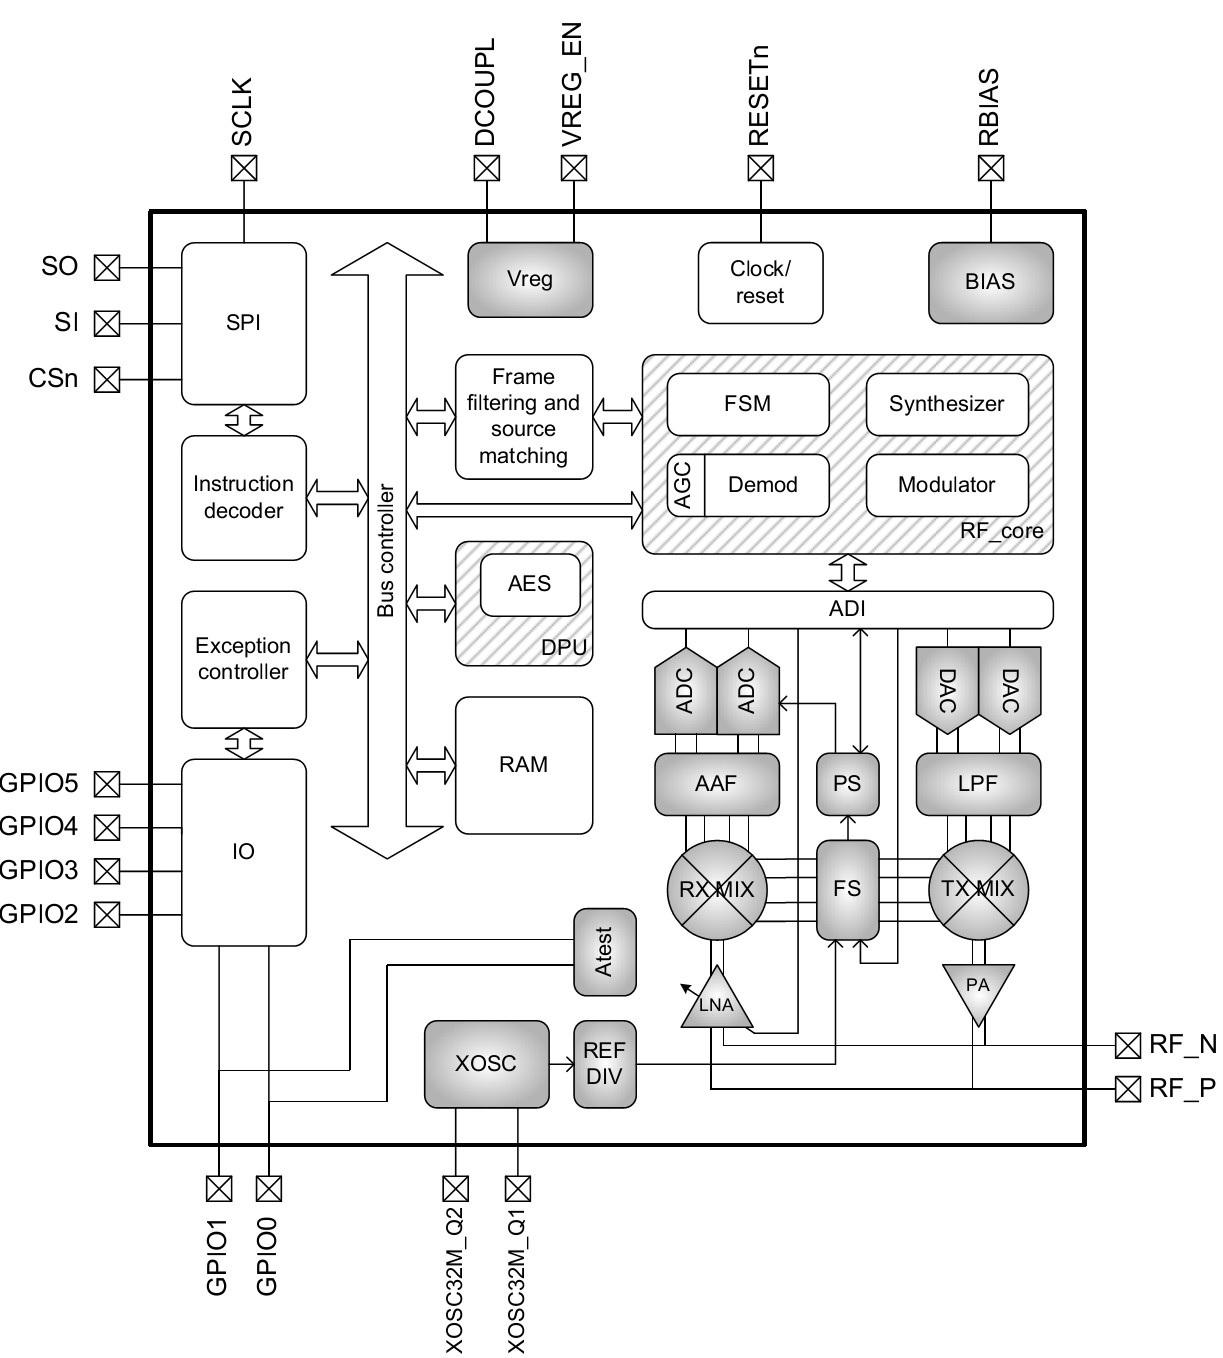
\includegraphics[height=1\textheight]{./imagenes/diagrama.jpg}
	\end{figure}	

\end{frame}

\begin{frame}{\textbf{Tx FIFO}}

	\begin{figure}[H]
		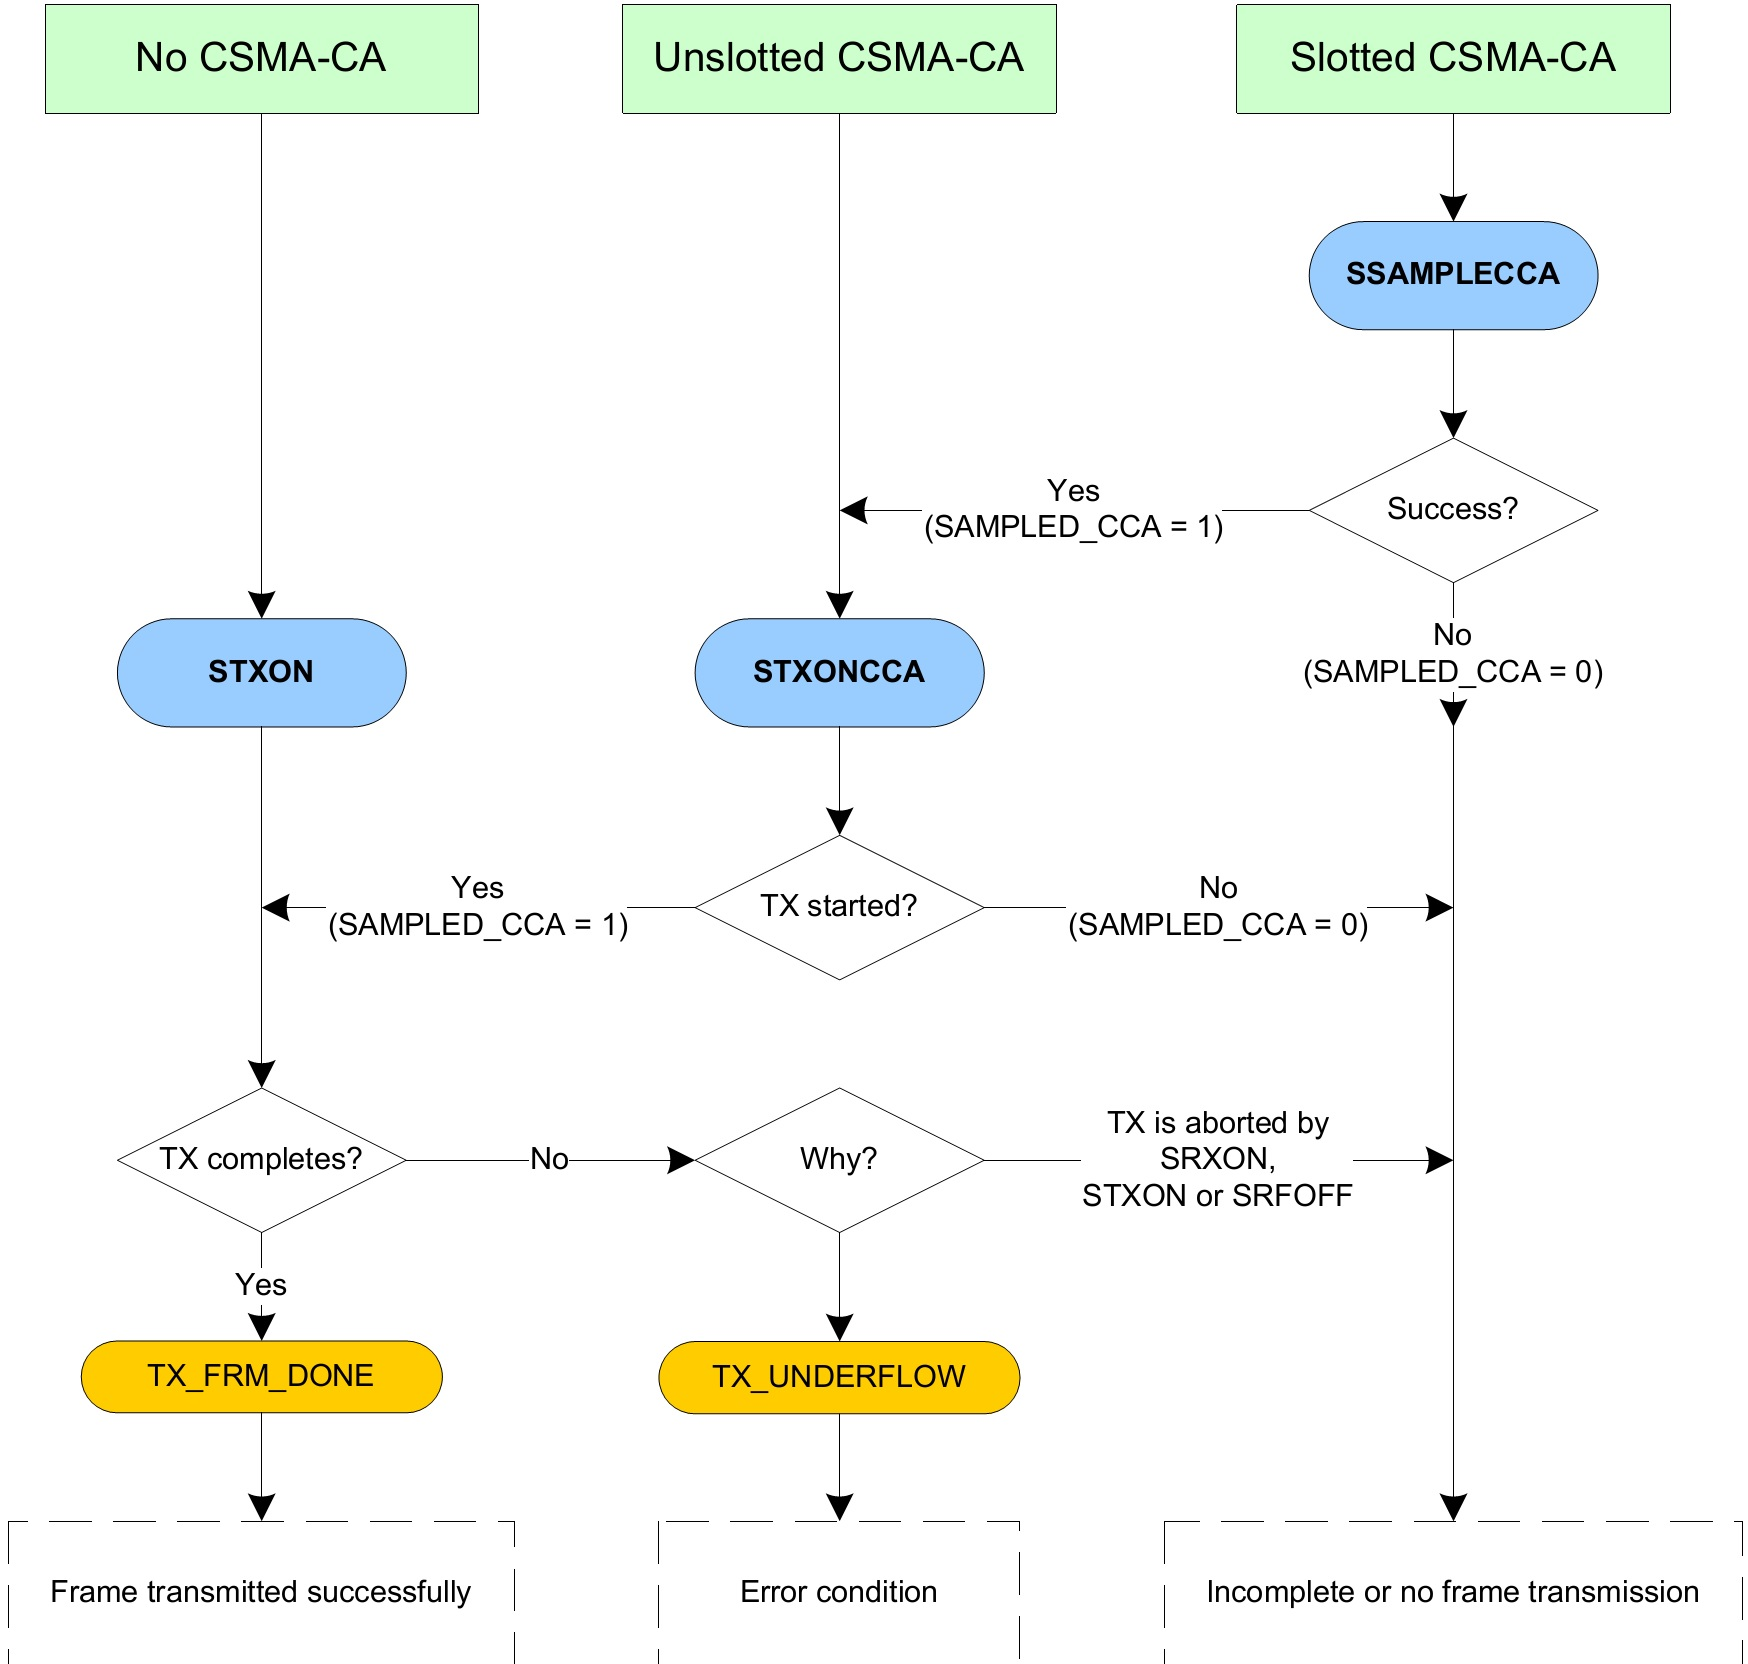
\includegraphics[height=1\textheight]{./imagenes/txfifo.jpg}
	\end{figure}	

\end{frame}

\begin{frame}{\textbf{Filtering Algorithm}}

	\begin{figure}[H]
		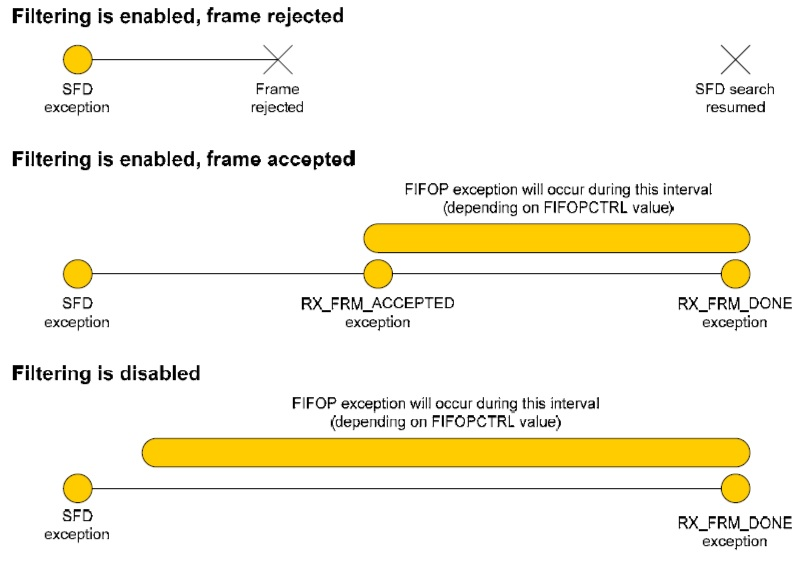
\includegraphics[height=1\textheight]{./imagenes/filtering.jpg}
	\end{figure}	

\end{frame}


\begin{frame}{\textbf{Matching Algorithm}}

	\begin{figure}[H]
		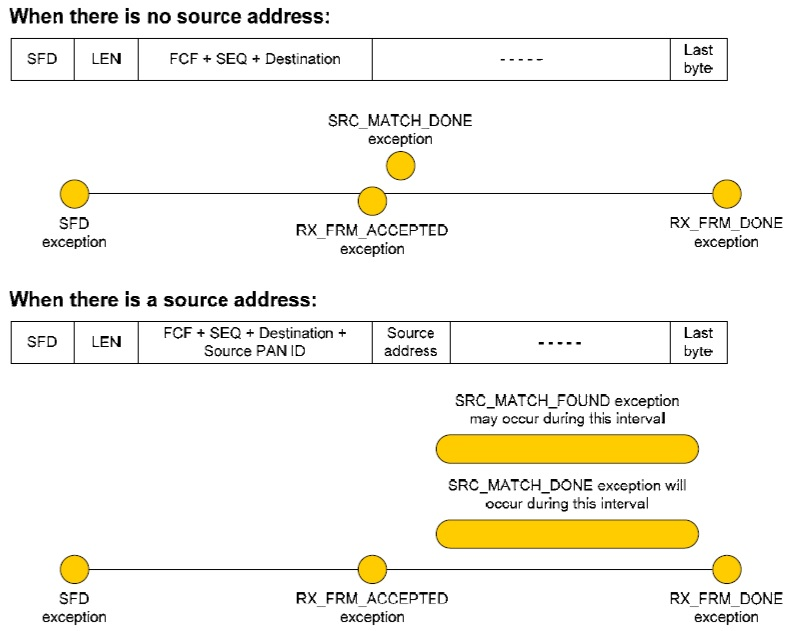
\includegraphics[height=1\textheight]{./imagenes/matching.jpg}
	\end{figure}	

\end{frame}


%\section[Problema]{Planteo del problema a resolver}
%
%\begin{frame}{\textbf{Planteo del problema a resolver}}
%\fontsize{18pt}{15}\selectfont
%	\begin{itemize}
%		\item {¿Qué hace falta medir?}
%		\vspace{20px}
%		\item ¿Qué hace falta controlar?
%		\vspace{20px}
%		\item ¿Sobre qué hace falta alertar?
%		\vspace{10px}
%	\end{itemize}
%\end{frame}
%
%\begin{frame}{\textbf{¿Qué hace falta medir? - Sensores}}
%\fontsize{14pt}{15}\selectfont
%
%\begin{minipage}[c]{1.0\linewidth}
%\begin{minipage}[c]{0.6\linewidth}
%      \centering
%      \begin{itemize}
%      	\item Temperatura
%		\vspace{10px}
%		\item pH
%		\vspace{10px}
%		\item Nivel de agua
%		\vspace{10px}
%		\item otros
%			\begin{itemize}
%				\item Conductividad
%				\item Nitratos
%				\item etc...
%			\end{itemize}
%	\end{itemize}
% \end{minipage}
%  \begin{minipage}[c]{0.35\linewidth}
%	\begin{figure}[H]
%	%	{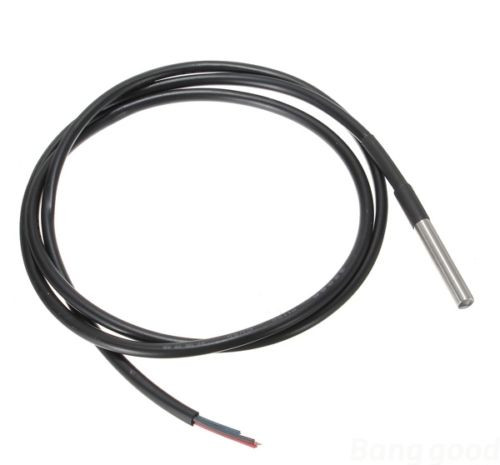
\includegraphics[width=1\textwidth]{./imagenes/sensor_temp}\vspace{5px}}
%	%	{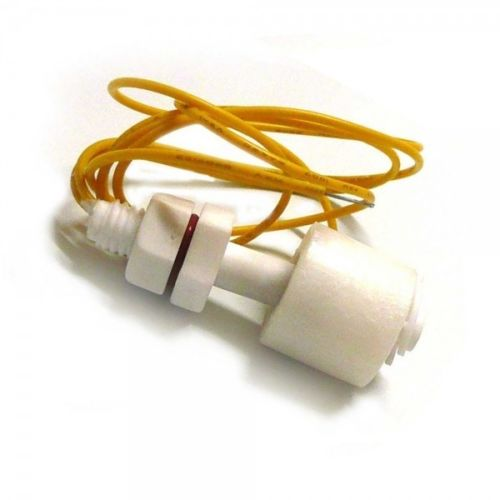
\includegraphics[width=1\textwidth]{./imagenes/sensor_nivel}}	
%	\end{figure}	  	  	
%  \end{minipage}
%\end{minipage}
%\end{frame}
%	
%
%\begin{frame}{\textbf{¿Qué hace falta controlar? - Actuadores}}
%\fontsize{14pt}{15}\selectfont
%\begin{minipage}[c]{1.0\linewidth}
%\begin{minipage}[c]{0.6\linewidth}
%      \centering
%	\begin{itemize}
%		\item Inyección de $O_2$/$CO_2$
%		\vspace{10px}
%		\item Iluminación
%		\vspace{10px}
%		\item Recambio de agua
%		\vspace{10px}
%		\item Calentadores
%		\vspace{10px}
%		\item Otros
%			\begin{itemize}
%				\item Dosificadores de alimento/nutrientes
%				\item Refrigeración
%				\item etc...
%			\end{itemize}
%	\end{itemize}
% \end{minipage}
%  \begin{minipage}[c]{0.35\linewidth}
%	\begin{figure}[H]
%	%	{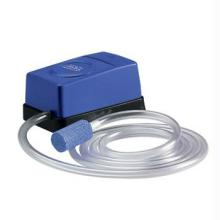
\includegraphics[width=1\textwidth]{./imagenes/actuador_pump}\vspace{5px}}
%	%	{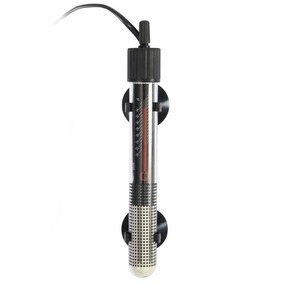
\includegraphics[width=1\textwidth]{./imagenes/actuador_heater}}	
%	\end{figure}	  	  	
%  \end{minipage}
%\end{minipage}
%\end{frame}
%
%\begin{frame}{\textbf{¿Sobre qué hace falta alertar? - Alarmas}}
%\fontsize{14pt}{15}\selectfont
%\begin{itemize}
%	\item Aviso de tarea periódica de mantenimiento
%	\vspace{10px}
%	\item Nivel de agua bajo/alto en tanques auxiliares
%	\vspace{10px}
%	\item Parámetro fuera de rango
%	\vspace{10px}
%	\item Falla de sensor
%	\vspace{10px}
%	\item Otros	
%\end{itemize}	
%\end{frame}
%
%\begin{frame}{\textbf{Soluciones existentes}}
%\fontsize{14pt}{15}\selectfont
%\vspace{-10px}
%	\begin{figure}
%	\begin{align*} 
%		{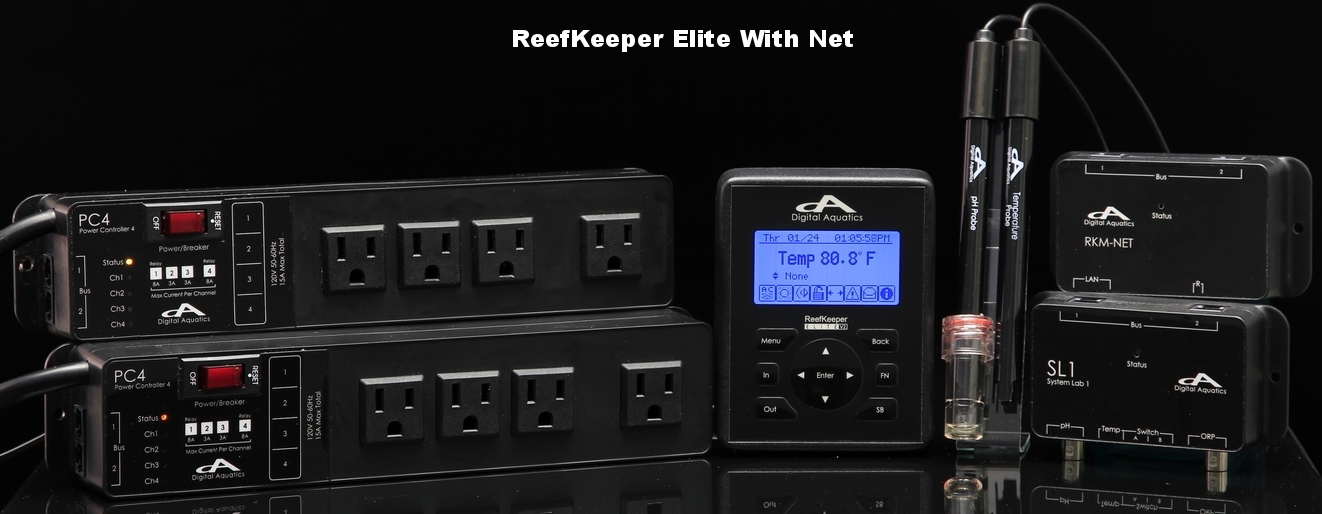
\includegraphics[width=.6\textwidth]{./imagenes/reefkeeper.JPG}}\\
%		\vspace{15px}
%		{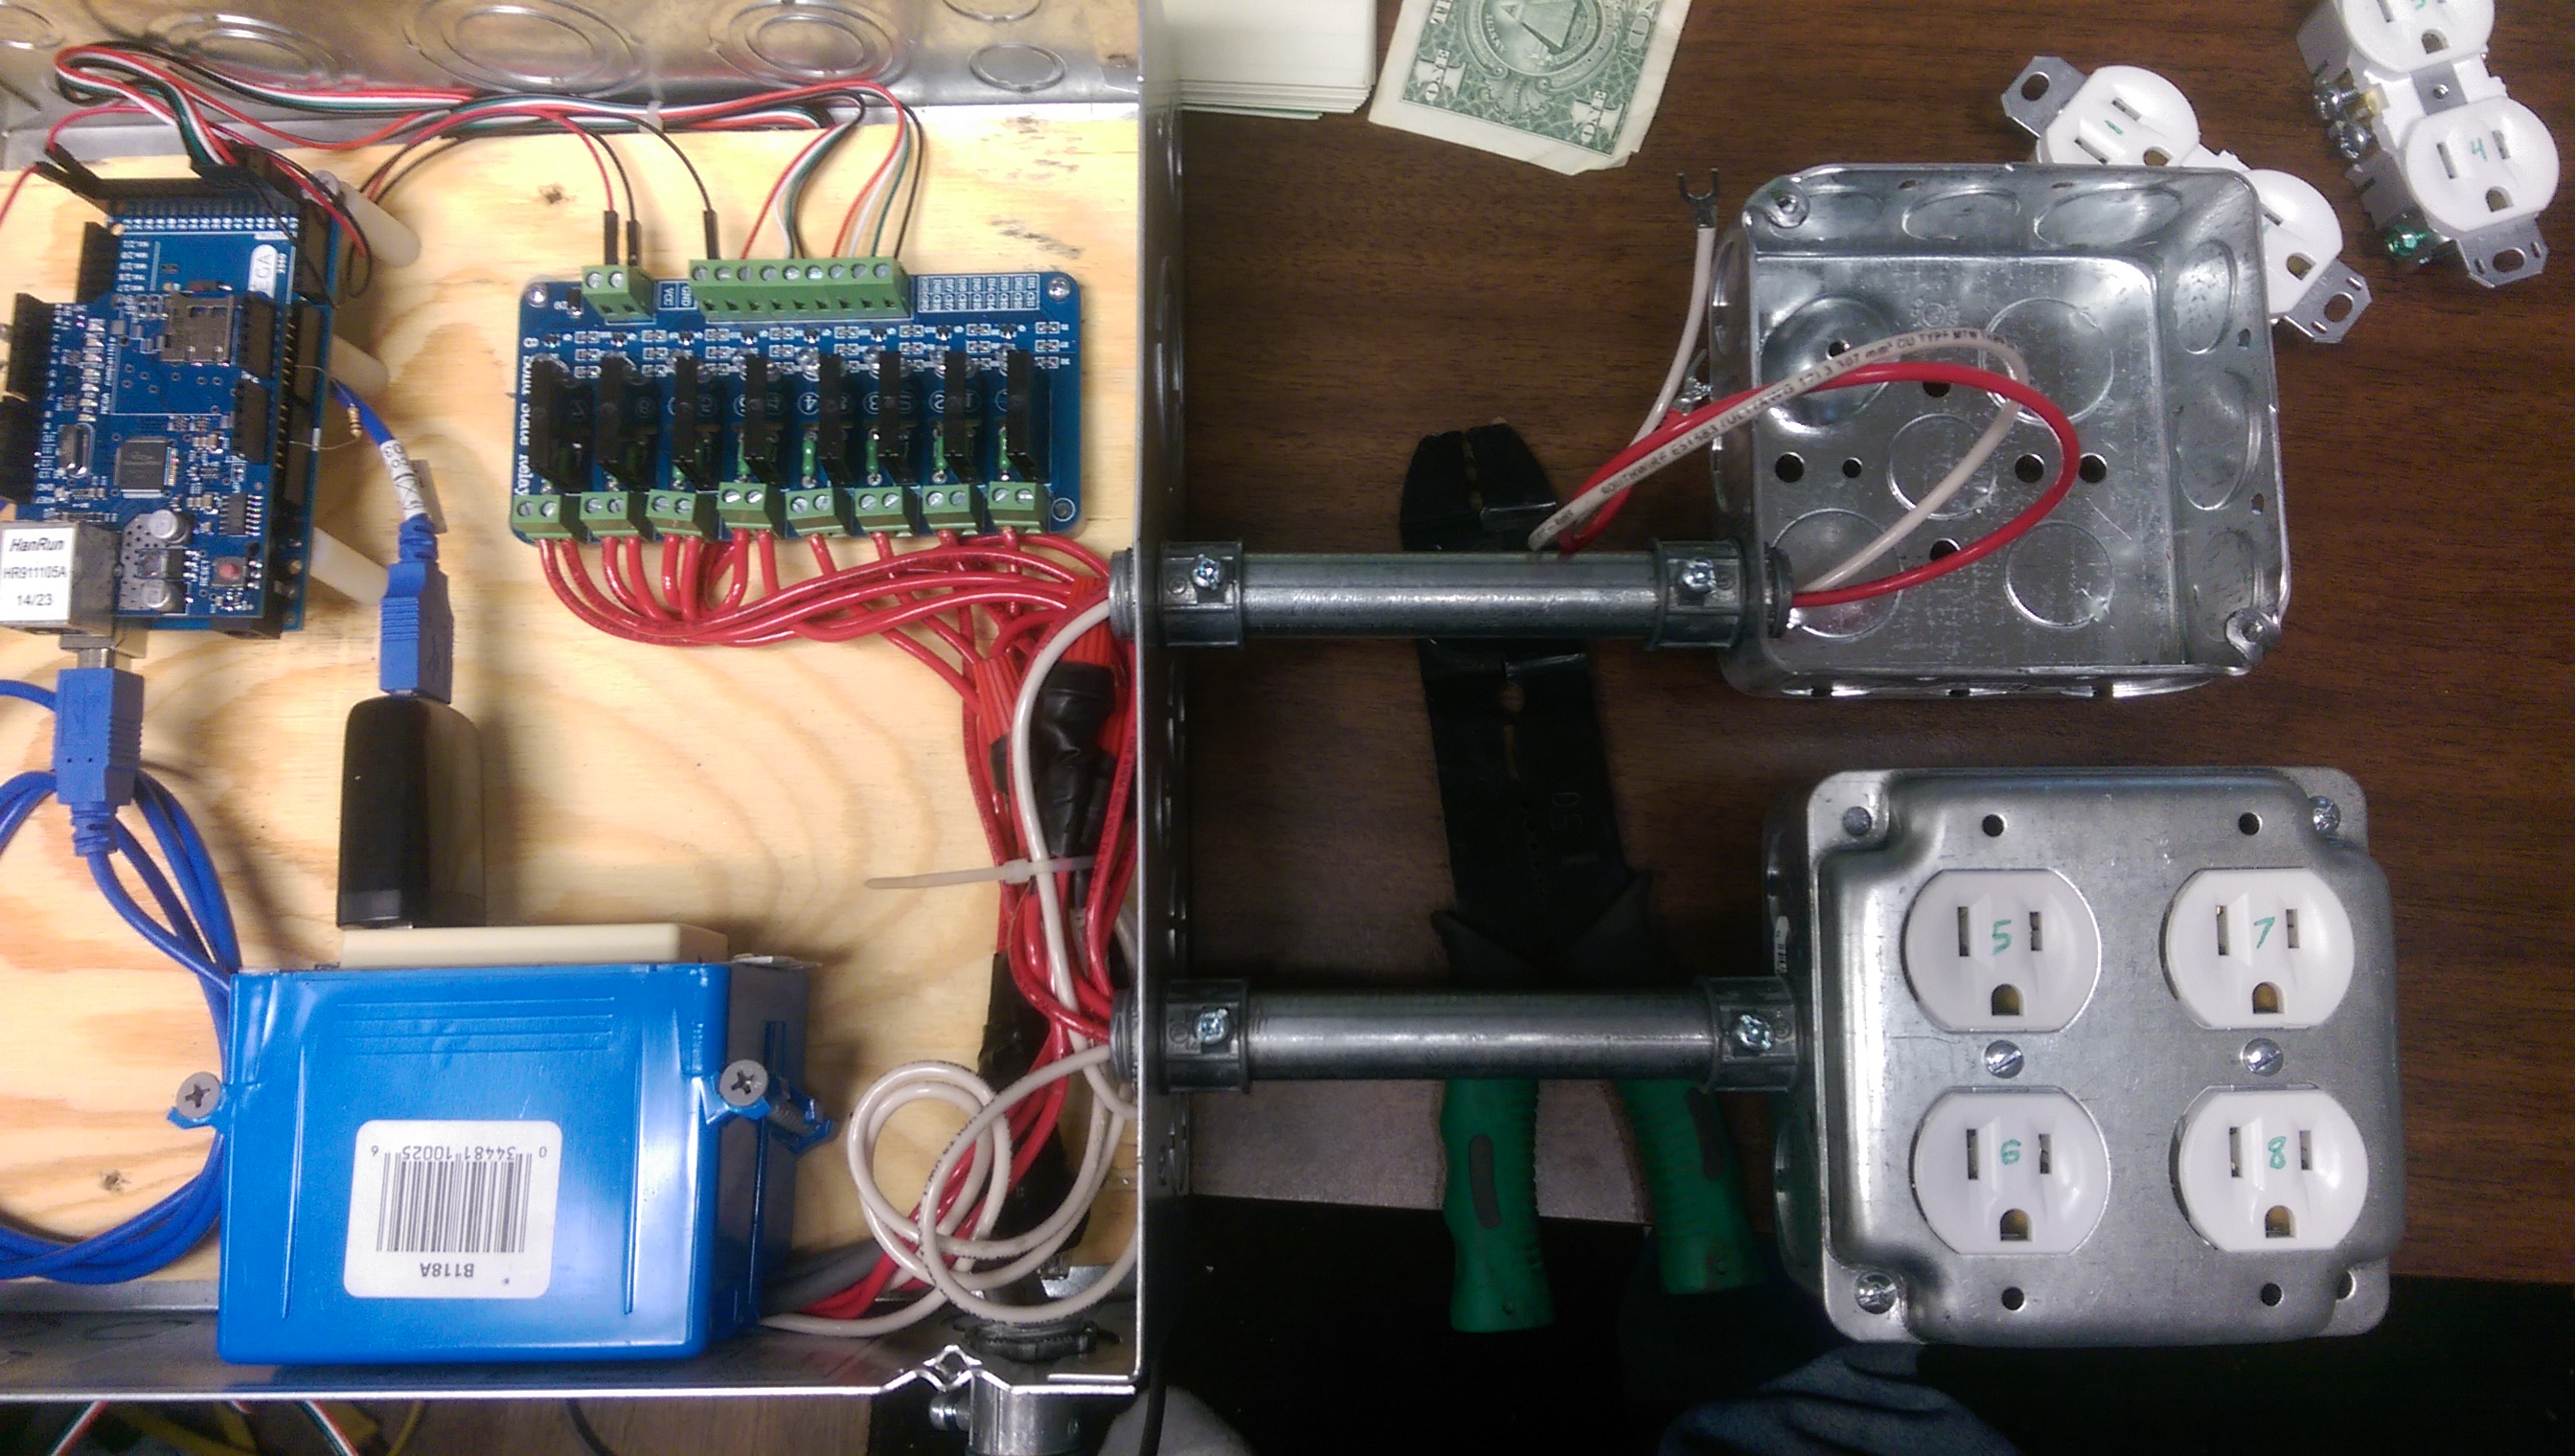
\includegraphics[width=.6\textwidth]{./imagenes/arduino.jpg}}
%	\end{align*}
%	\end{figure}	  	  	
%\end{frame}
%%
%
%
%


\section{Referencias}

\begin{frame}[t]{Referencias}
\begin{itemize}
	\item \href{http://ecee.colorado.edu/~liue/teaching/comm_standards/2015S_zigbee/802.15.4-2011.pdf}{Estándar IEEE 802.15.4:2011}
	\item \href{http://www.ieee802.org/15/pub/TG4.html}{IEEE 802.15 - Task Group 4 - Home Page}
	\item \href{	https://standards.ieee.org/about/get/802/802.15.html}{IEEE Get Program}
\end{itemize}
\end{frame}

%\begingroup
%\makeatletter
%\setlength{\hoffset}{-.5\beamer@sidebarwidth}
%\makeatother
%\begin{frame}[plain,noframenumbering]
%\fontsize{18pt}{15}\selectfont
%\begin{center}
%	MUCHAS GRACIAS POR SU ATENCIÓN\\
%	\vspace{2cm}
%	¿PREGUNTAS?
%	\begin{minipage}[c]{0.35\linewidth}
%		\begin{figure}[H]
%			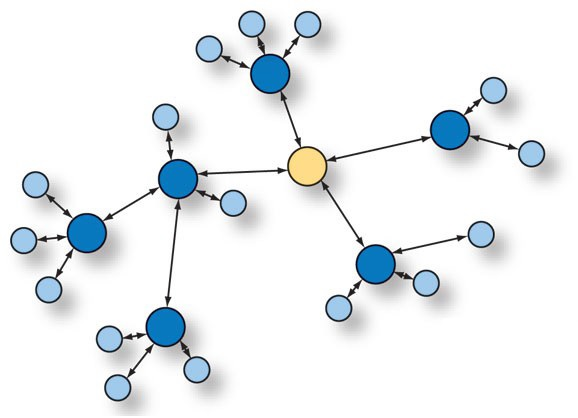
\includegraphics[width=1\textwidth]{./imagenes/red.jpg}
%		\end{figure}	  	  	
%	\end{minipage}
%\end{center}
%\end{frame}
%\endgroup

\end{document}
